\begin{frame}
    \titlepage
\end{frame}

\section{Introduction}

% FIXME: explain why the tree is structural; provide intuition why it's also the good structure

\begin{frame}
    \includegraphics[width=\textwidth]{ecosystem.pdf}
\end{frame}

\begin{frame}[fragile, t]
    \frametitle{What is Undefined Behavior ?}

    \begin{onlyenv}<1>
        Common pattern:
        \begin{itemize}
            \item for expressivity and performance the language introduces low level primitives \\
                (\texttt{std::mem::transmute}, pointer arithmetic, \texttt{Obj.magic}, ...),
            \item misuse of these primitives can interfere with compiler invariants \\
                (garbage collection, well-formedness of typed values, uniqueness, ...),
            \item guaranteeing deterministic behavior is
                \begin{itemize}
                    \item too expensive
                        (runtime bounds checks, type markers, ...)
                    \item not feasible
                        (undecidable at compile time)
                    \item or otherwise undesirable
                        (wasted optimization potential)
                \end{itemize}
        \end{itemize}
    \end{onlyenv}

    \begin{onlyenv}<2>
        \begin{alertblock}{Solution}
            Make it UB to misuse these constructs.\\
            If a compiler invariant is violated by a language primitive, the compiler can do literally anything.
        \end{alertblock}
        \begin{block}{UB as a contract}
            Deal between the programmer and the compiler: these primitives are
            dangerous, only use them if you really know what you are doing.
        \end{block}
        \begin{exampleblock}{\texttt{unsafe}}
            Already a selling point of Rust: \texttt{unsafe} is explicit.\\
            UB can only occur as a result of well-delimited blocks.
        \end{exampleblock}
    \end{onlyenv}
\end{frame}

\begin{frame}[fragile, t]
    \frametitle{Common examples}

    \begin{onlyenv}<1>
        Unchecked out-of-bounds accesses
        \begin{block}{Rust}
            \begin{lstlisting}[language=rust]
let v = { let x = [0]; unsafe { x.get_unchecked(1) } };
            \end{lstlisting}
        \end{block}

        \begin{block}{C}
            \begin{lstlisting}[language=c]
int* x = malloc(sizeof(int)); int v = x[1];
            \end{lstlisting}
        \end{block}
    \end{onlyenv}

    \begin{onlyenv}<2>
        Dereferencing null
        \begin{block}{Rust}
            \begin{lstlisting}[language=rust]
let v = unsafe { *(0 as *const u8) }
            \end{lstlisting}
        \end{block}

        \begin{block}{C}
            \begin{lstlisting}[language=c]
int v = *(int*)0
            \end{lstlisting}
        \end{block}
    \end{onlyenv}

    \begin{onlyenv}<3>
        Constructing an invalid value
        \begin{block}{Rust}
            \begin{lstlisting}[language=rust]
let x: bool = unsafe { std::mem::transmute(2) };
            \end{lstlisting}
        \end{block}

        \begin{block}{C}
            \begin{lstlisting}[language=c]
bool x = ((union { int i; bool b }){ .i = 2 }).b;
            \end{lstlisting}
        \end{block}
    \end{onlyenv}
\end{frame}

\begin{frame}[fragile, t]
    \frametitle{Pointer types in Rust}
    \begin{onlyenv}<1>
        \begin{lstlisting}[language=rust, escapechar=@]
// Raw pointers (unsafe)
*const T
*mut T
// (*const T @\(\sqsubset\)@ *mut T)

// References (safe)
&'a T // shared and immutable
&'a mut T // unique and mutable
// (&'a T @\(\sqsubset\)@ &'a mut T)
// ('a @\(\subset\)@ 'b @\(\Rightarrow\)@ &'a T @\(\sqsubset\)@ &'b T)
// ('a @\(\subset\)@ 'b @\(\Rightarrow\)@ &'a mut T @\(\sqsubset\)@ &'b mut T)

// Wrappers
UnsafeCell, Box, Unique, ...
        \end{lstlisting}
    \end{onlyenv}

    \begin{onlyenv}<2>
        Just like
        \begin{lstlisting}[language=rust]
// x: &mut bool
*x = 4;
        \end{lstlisting}
        is a type error (mismatched types \texttt{bool} and \texttt{u8}),
        \begin{lstlisting}[language=rust]
// x: &u8
*x = 4;
        \end{lstlisting}
        is also a type error (\texttt{\&\_} does not support assignment),
        and so is
        \begin{lstlisting}[language=rust]
// n: u8
let p = (&mut n, &mut n);
        \end{lstlisting}
        (impossible to satisfy lifetime constraints).\\

        Mutability and uniqueness are part of the type!\\
        Can we exploit that?
    \end{onlyenv}
\end{frame}

\begin{frame}[fragile, t]
    \frametitle{Is \texttt{\&mut} really unique ?}
    \begin{lstlisting}[language=rust]
let data: u64 = 0;
let r0: &mut u64 = &mut x;

let x: &mut u64 = unsafe { &mut *(r0 as *mut u64) };
let y: &mut u64 = unsafe { &mut *(r0 as *mut u64) };
*x += 1;
*y += 1;
    \end{lstlisting}
    Clearly \texttt{x} and \texttt{y} alias, even though they
    are both unrelated \texttt{\&mut}.

    \begin{onlyenv}<2->
        \begin{block}{\texttt{unsafe} can violate compiler invariants}
            \texttt{unsafe} code can violate uniqueness (and well-formedness)
            guarantees, so the compiler cannot rely on them for optimizations.
        \end{block}
    \end{onlyenv}
\end{frame}

\begin{frame}[fragile, t]
    \frametitle{A motivating example for Aliasing UB}
    \begin{lstlisting}[language=rust]
fn foo(x: &mut u64) {
    let val = *x;
    *x = 42;
    opaque();
    *x = val;
}
    \end{lstlisting}
    optimized into
    \begin{lstlisting}[language=rust]
fn foo(x: &mut u64) {
    opaque();
}
    \end{lstlisting}
    Well-typedness of any program that calls \texttt{foo} implies uniqueness
    of \texttt{x} during the execution of \texttt{foo}: \texttt{opaque} cannot mutate \texttt{x}!\\
    \begin{onlyenv}<2->
    ...except if the user uses \texttt{unsafe} to violate uniqueness \\
    \end{onlyenv}
    \begin{onlyenv}<3>
    ...which we are going to assume does not happen: violating uniqueness is UB!
    \end{onlyenv}
\end{frame}


\begin{frame}[fragile, t]
    \frametitle{How much UB is enough ? Too much ?}
    \vspace{-1em}
    \begin{figure}
        \makebox[\textwidth][c]{
            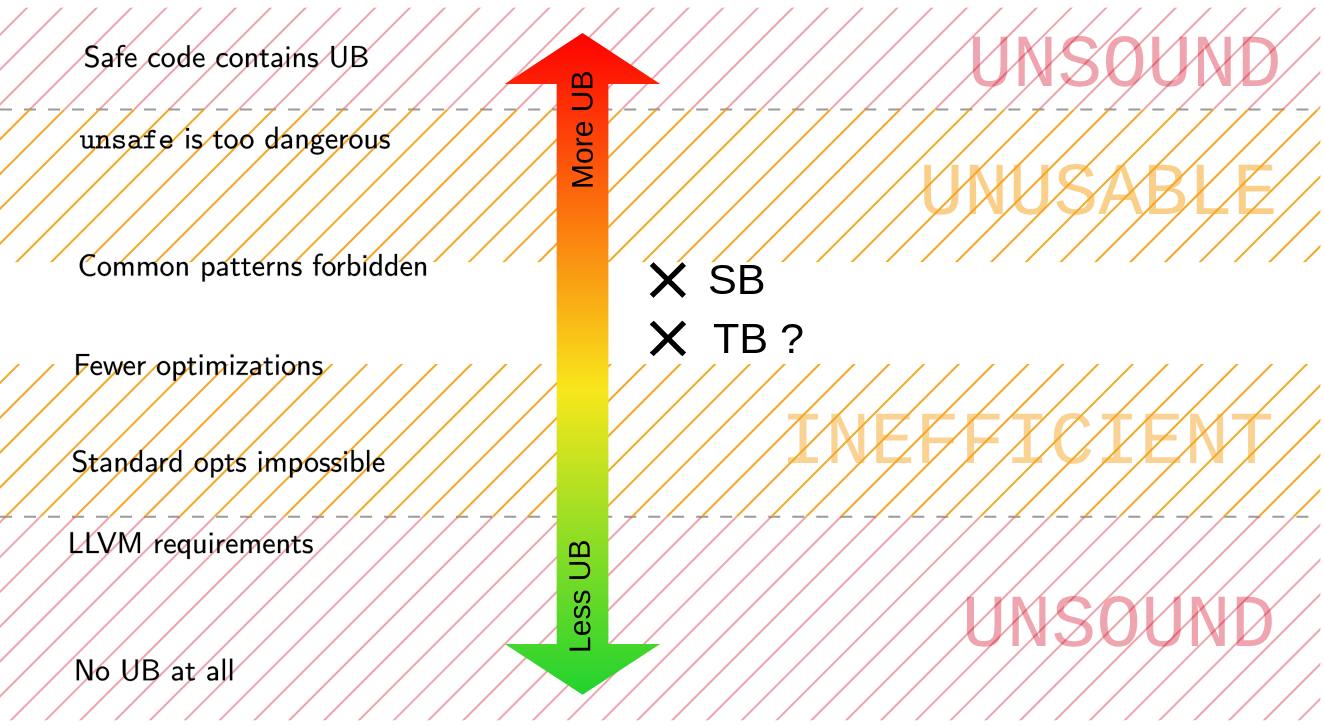
\includegraphics[width=13cm]{how-much-ub.png}
        }
    \end{figure}
\end{frame}

\begin{frame}[t]
    \frametitle{Tree Borrows: specification and detection of pointer aliasing UB}
    \begin{alertblock}{Starting observation}
        Proper usage of pointers (lifetime inclusion and inheritance of mutability) follows a tree discipline.
        \begin{itemize}
            \item when pointer dies, so do its children
            \item when pointer requires uniqueness, remove other branches
        \end{itemize}
    \end{alertblock}
    \begin{block}{Key ideas}
        \begin{itemize}
            \item per-location tracking of pointers
            \item each pointer has permissions
            \item on each reborrow a new identifier is added as a leaf of the tree
            \item a pointer can be used if its permission allows it (to be defined)
            \item using a pointer kills incompatible (to be defined) pointers
        \end{itemize}
    \end{block}
\end{frame}

